% Slide 10 — privacy.
%
% The swap is the slide: two hosted speech APIs struck out, two open models in
% their place. Drawn rather than described, because "we run speech locally" is
% a sentence and a crossed-out vendor is an argument.
%
% Only STT and TTS are replaced. The reasoning model is still a hosted call, so
% the claim is about the participant's recorded voice and is written that way —
% "their voice never leaves", not "nothing leaves".
%
% No filenames anywhere: a store is named by what it holds.
\documentclass[border=0pt]{standalone}
% Figure preamble: the shared base plus a transparent page background, so a
% figure composites onto the slide ground instead of carrying a white box.
% Shared preamble for every Reconmed figure and slide.
\usepackage{xcolor}
\usepackage{graphicx}
\usepackage{tikz}
\usetikzlibrary{positioning,calc,fit,backgrounds,shapes.misc,arrows.meta,decorations.pathreplacing}

% Reconmed — presentation palette.
%
% A green medical theme, derived from the product's tokens (frontend/src/styles/
% tokens.css) but with the brand moved to a deep clinical green.
%
% The product's colour rule survives the rebrand unchanged: warm hues (alarm,
% caution) are reserved for prohibited findings and low confidence — never for
% change types. Change types stay cool and are kept off the brand green so the
% brand and the "add" state do not blur together.
\definecolor{ground}{HTML}{EFF4F0}
\definecolor{surf}{HTML}{FFFFFF}
\definecolor{surfii}{HTML}{F6FAF7}
\definecolor{surfiii}{HTML}{E5EDE7}

\definecolor{line}{HTML}{DBE5DD}
\definecolor{lineii}{HTML}{C1D1C4}
\definecolor{lineiii}{HTML}{92A796}

\definecolor{ink}{HTML}{10231A}
\definecolor{inkii}{HTML}{3B4F43}
\definecolor{inkiii}{HTML}{66796D}
\definecolor{inkiv}{HTML}{92A796}

% the brand green
\definecolor{brand}{HTML}{14532D}
\definecolor{brandii}{HTML}{1B6B3A}
\definecolor{brandwash}{HTML}{E8F2EA}

% the participant side of the call — cool and neutral, so the agent's green
% is the only brand colour on the slide
\definecolor{patient}{HTML}{4E6570}

% change types — cool, deliberately unalarming
\definecolor{add}{HTML}{15803D}
\definecolor{stop}{HTML}{6A4C93}
\definecolor{modify}{HTML}{1F5FA8}
\definecolor{same}{HTML}{6B7C70}

% the one loud thing
\definecolor{alarm}{HTML}{C2190B}
\definecolor{alarmink}{HTML}{A3170C}
\definecolor{alarmdim}{HTML}{F1B9B2}
\definecolor{alarmwash}{HTML}{FDF3F1}

% low confidence — dim gold, never red
\definecolor{caution}{HTML}{8A6206}

\definecolor{accept}{HTML}{15803D}
% Rejected is a decision, not an alarm: kept neutral so red stays reserved for
% prohibited findings.
\definecolor{reject}{HTML}{5F6B72}

% Type for the deck.
%
% Two families: Montserrat for headings, big numbers and the wordmark — a
% geometric sans that reads as a health brand — over Open Sans for everything
% else. Keeping the body on Open Sans matters: the dense technical slides were
% measured against it, so the small type does not reflow under the rebrand.
\usepackage{fontspec}
\defaultfontfeatures{Ligatures=TeX}
\setsansfont{Open Sans}
\newfontfamily\displayfont{Montserrat}
\renewcommand{\familydefault}{\sfdefault}

% Shared TikZ styles. Every figure draws in millimetres (x=1mm,y=1mm) on a
% 160x90 canvas, so these sizes are literal.
%
% No blank lines may appear inside the \tikzset below: a blank line is \par,
% and the key parser will not tolerate it.
\tikzset{
  panel/.style     = {draw=line, fill=surf,   line width=0.4pt, rounded corners=2pt},
  panelgray/.style = {draw=line, fill=surfii, line width=0.4pt, rounded corners=2pt},
  screen/.style    = {draw=line, fill=surf,   line width=0.5pt, rounded corners=2.5pt},
  hair/.style      = {draw=line,   line width=0.4pt},
  hairii/.style    = {draw=lineii, line width=0.5pt},
  dimbar/.style    = {fill=line,   rounded corners=0.6pt},
  dimbarsm/.style  = {fill=lineii, rounded corners=0.5pt},
  lab/.style       = {font=\fontsize{7}{8.5}\selectfont\sffamily\color{inkiii}, inner sep=0pt, outer sep=0pt},
  val/.style       = {font=\fontsize{9}{11}\selectfont\sffamily\color{ink},    inner sep=0pt, outer sep=0pt},
  valb/.style      = {font=\fontsize{9}{11}\selectfont\sffamily\bfseries\color{ink}, inner sep=0pt, outer sep=0pt},
  code/.style      = {font=\fontsize{7}{8.5}\selectfont\ttfamily\color{inkiii}, inner sep=0pt, outer sep=0pt},
  tag/.style       = {font=\fontsize{5.6}{6.5}\selectfont\sffamily\bfseries, inner xsep=1.3mm, inner ysep=0.7mm, rounded corners=1.4pt},
  pill/.style      = {font=\fontsize{6.4}{7.5}\selectfont\sffamily\bfseries, inner xsep=1.5mm, inner ysep=0.85mm, rounded corners=1.5pt},
  headline/.style  = {font=\fontsize{12}{14}\selectfont\sffamily\bfseries\color{ink}, anchor=west, inner sep=0pt, outer sep=0pt},
  subline/.style   = {font=\fontsize{7.5}{9}\selectfont\sffamily\color{inkii}, anchor=west, inner sep=0pt, outer sep=0pt},
  cardlab/.style   = {font=\fontsize{6.4}{7.5}\selectfont\sffamily\color{inkiii}, anchor=west, inner sep=0pt, outer sep=0pt},
  num/.style       = {font=\fontsize{22}{23}\selectfont\sffamily\bfseries\color{ink}, anchor=west, inner sep=0pt, outer sep=0pt},
  flow/.style      = {-{Stealth[length=1.5mm,width=1.2mm]}, draw=lineii, line width=0.7pt},
}

% The conmed mark.
%
% Concept: two records — the log on file, and what the participant said —
% converging into a single reconciled line. Drawn once as a standalone asset
% (shared/marks/conmed.tex) so it scales cleanly: PDF inclusion scales the
% strokes, which TikZ scope scaling would not.
\newcommand{\conmedmark}[1][16mm]{
\includegraphics[height=#1]{shared/marks/conmed.pdf}}


\AtBeginDocument{\ifdefined\nopagecolor\nopagecolor\fi}

\begin{document}
\hyphenpenalty=10000\exhyphenpenalty=10000

% A vendor chip with a line through it.
\newcommand{\struck}[3]{% #1 x  #2 y  #3 label
  \fill[surfii, rounded corners=2pt] (#1,#2) rectangle (#1+34,#2+13);
  \draw[line, line width=0.4pt, rounded corners=2pt] (#1,#2) rectangle (#1+34,#2+13);
  \node[anchor=center] at (#1+9,#2+6.5) {
\includegraphics[height=3.6mm]{shared/marks/deepgram.pdf}};
  \node[anchor=west, font=\fontsize{6.4}{7.7}\selectfont\sffamily\color{inkiii}] at (#1+15,#2+6.5) {#3};
  \draw[alarm, line width=0.9pt] (#1+13.5,#2+6.5) -- (#1+31,#2+6.5);
}

% The open model that replaced it.
\newcommand{\localmodel}[4]{% #1 x  #2 y  #3 model  #4 provenance
  \fill[brand!8!white, rounded corners=2pt] (#1,#2) rectangle (#1+44,#2+13);
  \draw[brand, line width=0.6pt, rounded corners=2pt] (#1,#2) rectangle (#1+44,#2+13);
  \node[anchor=west, font=\fontsize{7.4}{9}\selectfont\sffamily\bfseries\color{ink}] at (#1+4,#2+8.6) {#3};
  \node[anchor=west, font=\fontsize{5.6}{6.8}\selectfont\sffamily\color{inkii}] at (#1+4,#2+4.2) {#4};
}

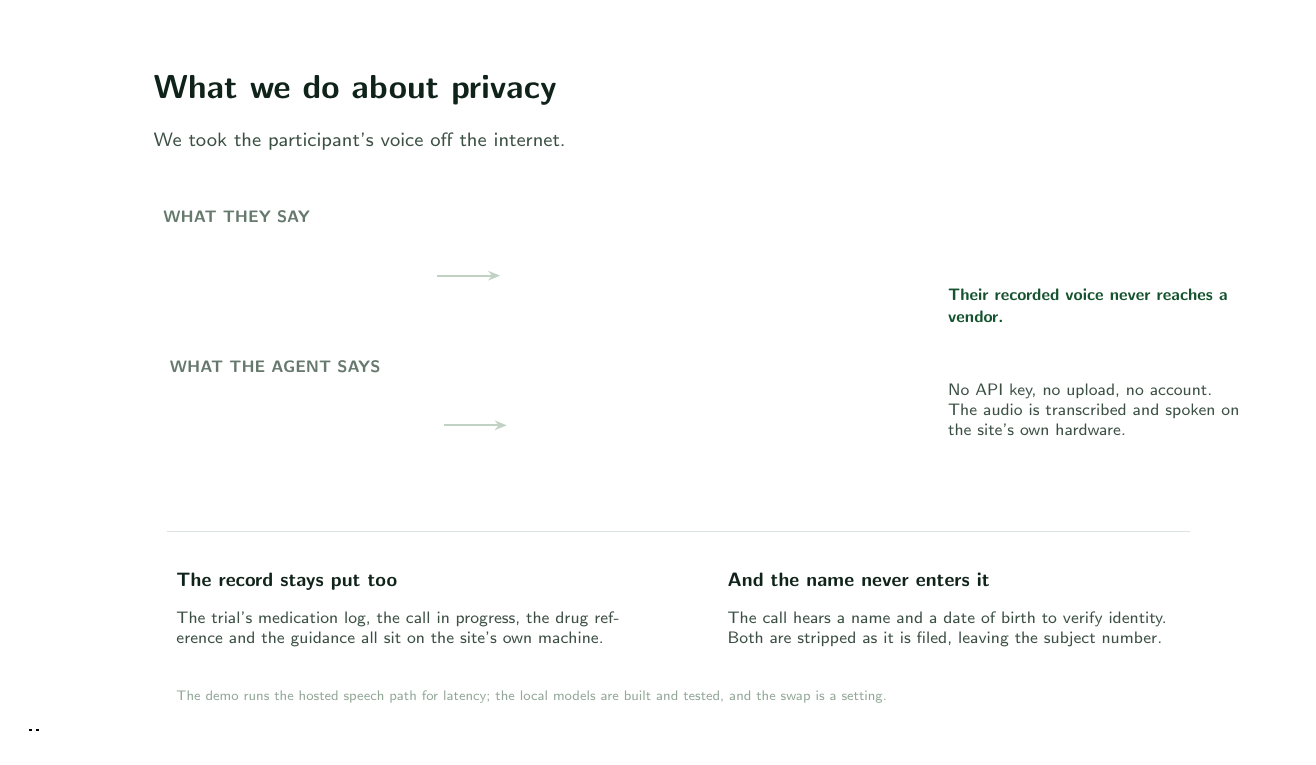
\begin{tikzpicture}[x=1mm,y=1mm]
\path[use as bounding box] (0,0) rectangle (160,90);

\node[headline] at (16,82) {What we do about privacy};
\node[subline]  at (16,75.5) {We took the participant's voice off the internet.};

% ---- the swap -----------------------------------------------------------
\node[anchor=west, font=\fontsize{5.6}{6.8}\selectfont\sffamily\bfseries\color{inkiii}] at (16,66) {WHAT THEY SAY};
\struck{16}{52}{speech-to-text}
\draw[flow] (52,58.5) -- (60,58.5);
\localmodel{64}{52}{Parakeet 0.6B}{NVIDIA \textperiodcentered\ open weights, on CPU}

\node[anchor=west, font=\fontsize{5.6}{6.8}\selectfont\sffamily\bfseries\color{inkiii}] at (16,47) {WHAT THE AGENT SAYS};
\struck{16}{33}{text-to-speech}
\draw[flow] (52,39.5) -- (60,39.5);
\localmodel{64}{33}{Qwen3-TTS 0.6B}{Alibaba \textperiodcentered\ open weights, on CPU}

\node[anchor=north west, font=\fontsize{6.4}{7.8}\selectfont\sffamily\bfseries\color{brand}, align=left, text width=38mm] at (114,58)
  {Their recorded voice never reaches a vendor.};
\node[anchor=north west, font=\fontsize{5.8}{7.2}\selectfont\sffamily\color{inkii}, align=left, text width=38mm] at (114,46)
  {No API key, no upload, no account. The audio is transcribed and spoken on the site's own hardware.};

% ---- the other two answers ---------------------------------------------
\draw[line, line width=0.5pt] (16,26) -- (146,26);

\node[anchor=north west, font=\fontsize{6.6}{8}\selectfont\sffamily\bfseries\color{ink}] at (16,22)
  {The record stays put too};
\node[anchor=north west, font=\fontsize{5.8}{7.2}\selectfont\sffamily\color{inkii}, align=left, text width=58mm] at (16,17)
  {The trial's medication log, the call in progress, the drug reference and the guidance all sit on the site's own machine.};

\node[anchor=north west, font=\fontsize{6.6}{8}\selectfont\sffamily\bfseries\color{ink}] at (86,22)
  {And the name never enters it};
\node[anchor=north west, font=\fontsize{5.8}{7.2}\selectfont\sffamily\color{inkii}, align=left, text width=58mm] at (86,17)
  {The call hears a name and a date of birth to verify identity. Both are stripped as it is filed, leaving the subject number.};

\node[anchor=west, font=\fontsize{5.4}{6.5}\selectfont\sffamily\color{inkiv}] at (16,5)
  {The demo runs the hosted speech path for latency; the local models are built and tested, and the swap is a setting.};

\end{tikzpicture}
\end{document}
